\section{Auswertung}
\label{sec:Auswertung}
Alle Berechnungen werden mit dem Programm \glqq Numpy" \cite{numpy}, die Unsicherheiten mit dem Modul \glqq Uncertainties" \cite{uncertainties}, die Ausgleichsrechnungen mit dem Modul \glqq Scipy" \cite{scipy} durchgeführt und die grafischen Darstellungen über das Modul \glqq Matplotlib" \cite{matplotlib} erstellt.



\subsection{Vertikales B-Feld}

Um die vertikale Komponente des Erdmagnetfeldes zu kompensieren, wird dem ein Gegenfeld einer Flussdichte von $B_v=\SI{35.25}{\micro\tesla}$ entgegengesetzt.


\subsection{B-Feld-Resonanzen}
Die Messung erfolgt gemäß dem in der Durchführung beschriebenen Ablauf. Die jeweiligen Resonanz-Positionen werden über Drehung des Potenziometers erreicht. 
Aus der Anzahl der Drehungen lässt sich der jeweils fließende Strom bestimmen. 
Dabei entspricht eine Umdrehung für die Sweep- und Vertilalfeld-Spulen einen Strom von $I=\SI{0.1}{\ampere}$ und für die Horizontalfeld-Spule einen Strom von $I=\SI{0.3}{\ampere}$. 
Aus den Strömen lassen sich die von den Helmholtzspulenpaaren erzeugten Magnetfelder über
\begin{equation}
    B_{\text{Helmholtz}} = \frac{8}{\sqrt{125}}\frac{\mu_0 N I}{R}
\end{equation}
berechnen. Die Summe aus Sweep- und Horizontalfeld ergibt die gesamte magnetische Flussdichte.
Die Ströme und die Flussdichten der Resonanzen sind der Tabelle \ref{tab:Resonanz} zu entnehmen. 

\begin{table}
    \centering
    \caption{}
    \label{tab:Resonanz}
    \sisetup{table-format = 1.2}
    \begin{tabular}[h]{S | S S S| S S S|} 
        \toprule
        & \multicolumn{3}{c}{$^{87}$Rb} & \multicolumn{3}{c}{$^{85}$Rb} \\
        \cmidrule(lr){2-4}\cmidrule(lr){5-7}
        $f \mathbin{/} \si{\kilo\hertz}$ & $I_{Sweep} \mathbin{/} \si{\ampere}$ & $I_{Hori.} \mathbin{/} \si{\ampere}$ & $B_{Summe} \mathbin{/} \si{\micro\tesla}$ & $I_{Sweep} \mathbin{/} \si{\ampere}$ & $I_{Hori.} \mathbin{/} \si{\ampere}$ & $B_{Summe} \mathbin{/} \si{\micro\tesla}$ \\
        \midrule
        100     &    0.65 &  0.77  &   39.23   &  0.00 &  0.00  &  46.35    \\
        200     &    0.43 &  0.67  &   52.14   &  0.03 &  0.03  &  66.44    \\
        300     &    0.67 &  1.02  &   66.50   &  0.03 &  0.03  &  87.68    \\
        400     &    0.54 &  0.97  &   85.21   &  0.06 &  0.06  & 111.40    \\
        500     &    0.34 &  0.90  &   99.45   &  0.09 &  0.09  & 133.24    \\
        600     &    0.13 &  0.84  &  113.08   &  0.12 &  0.12  & 155.99    \\
        700     &    0.20 &  1.03  &  122.69   &  0.13 &  0.13  & 172.60    \\
        800     &    0.25 &  1.02  &  141.31   &  0.14 &  0.16  & 198.12    \\
        900     &    0.31 &  0.84  &  155.39   &  0.16 &  0.19  & 219.13    \\
        1000    &    0.16 &  0.82  &  167.21   &  0.18 &  0.22  & 238.91    \\
        \bottomrule
    \end{tabular}
\end{table}
An den Resonanzen muss der Zusammenhang aus Gleichung REF gelten.
Dieser lässt sich unter Berücksichtigung eines Untergrundfeldes zu einer Geradengleichung der Form 
\begin{equation}
    \label{eq:B}
    B(f) = \underbrace{\frac{h}{\mu_B g_F}}_{=a}f + b
\end{equation}
umstellen.

\begin{figure}
    \centering
    \includegraphics[width=.9\textwidth]{build/B_Felder.pdf}
    \caption{Gemessene B-Felder der Resonanzen in Abhängigkeit der jeweiligen RF-Feld-Frequenzen für beide Rb-Isotope. Anhand der Messwerte lassen sich Ausgleichsgeraden berechnen.}
    \label{fig:Resonanz}
\end{figure}

In grafischer Darstellung (Abbildung \ref{fig:Resonanz}) lässt sich dieser lineare Zusammenhang zwischen der magnetischen Flussdichte und der Frequenz des RF-Feldes erkennen.
Es lässt sich eine Ausgleichsrechnung der Geraden aus Gleichung \eqref{eq:B} durchführen.
Die Ergebnisse dieser Rechnung ergeben sich für $^{87}$Rb zu  
\begin{align*}
    a_{87} = & \SI{0.1439(23)}{\micro\tesla\per\kilo\hertz} \\
    b_{87} = &\SI{25.1(14)}{\micro\tesla} 
\end{align*}
und für $^{85}$Rb zu
\begin{align*}
    a_{85} =& \SI{0.2158(18)}{\micro\tesla\per\kilo\hertz} \\
    b_{85} =&  \SI{24.3(11)}{\micro\tesla}.
\end{align*}
Der konstante Untergrund lässt sich hauptsächlich auf die verbleibende horizontalkomponente des Erdmagnetfeldes zurückführen. 



Aus den Steigungen der Ausgleichsgeraden lässt sich der jeweilige g-Faktor bestimmen.
Dazu wird die Steigung $a$ aus Gleichung \eqref{eq:B} nach dem g-Faktor $g_F$ umgeformt.
So lässt sich über
\begin{equation}
    g_F = \frac{h}{\mu_B a}
\end{equation}
der g-Faktor für $^{87}$Rb zu 
\begin{align*}
    g_F = \num{0.496(8)}
\end{align*}
und für $^{85}$Rb zu 
\begin{align*}
    g_F=\num{0.3311(27)}
\end{align*}
bestimmen.

Da der g-Faktor im Wesentlichen nur von der Drehimpuls-, Elektronenspin- und der Kernspinquantenzahl abhängt, lässt sich bei gegebenen $l$, $s$ und g-Faktor der jeweilige Kernspin $I$ über Gleichung REF bestimmen.
Da nach dem optischen Pumpen hauptsächlich Zustände aus der $^2S_{\frac{1}{2}}$-Schale besetzt sind, belaufen sich die Quantenzahlen auf $l=0$ und $s=\nicefrac{1}{2}$.
Wird die Gleichung REF mit diesen Quantenzahlen passend umgeformt, lässt sich der Kernspin über
\begin{equation}
    I = \frac{1}{g_F}-\frac{1}{2}
\end{equation}
berechnen.
Mit den ermittelten g-Faktoren ergibt sich für $^{87}$Rb ein Kernspin von
\begin{equation*}
    I_{87} = \num{1.514(33)}
\end{equation*}
und für $^{85}$Rb ein Kernspin von
\begin{equation*}
    I_{85} = \num{2.520(25)}. 
\end{equation*}



\subsection{Isotopenverhältnis}

\begin{figure}
    \centering
    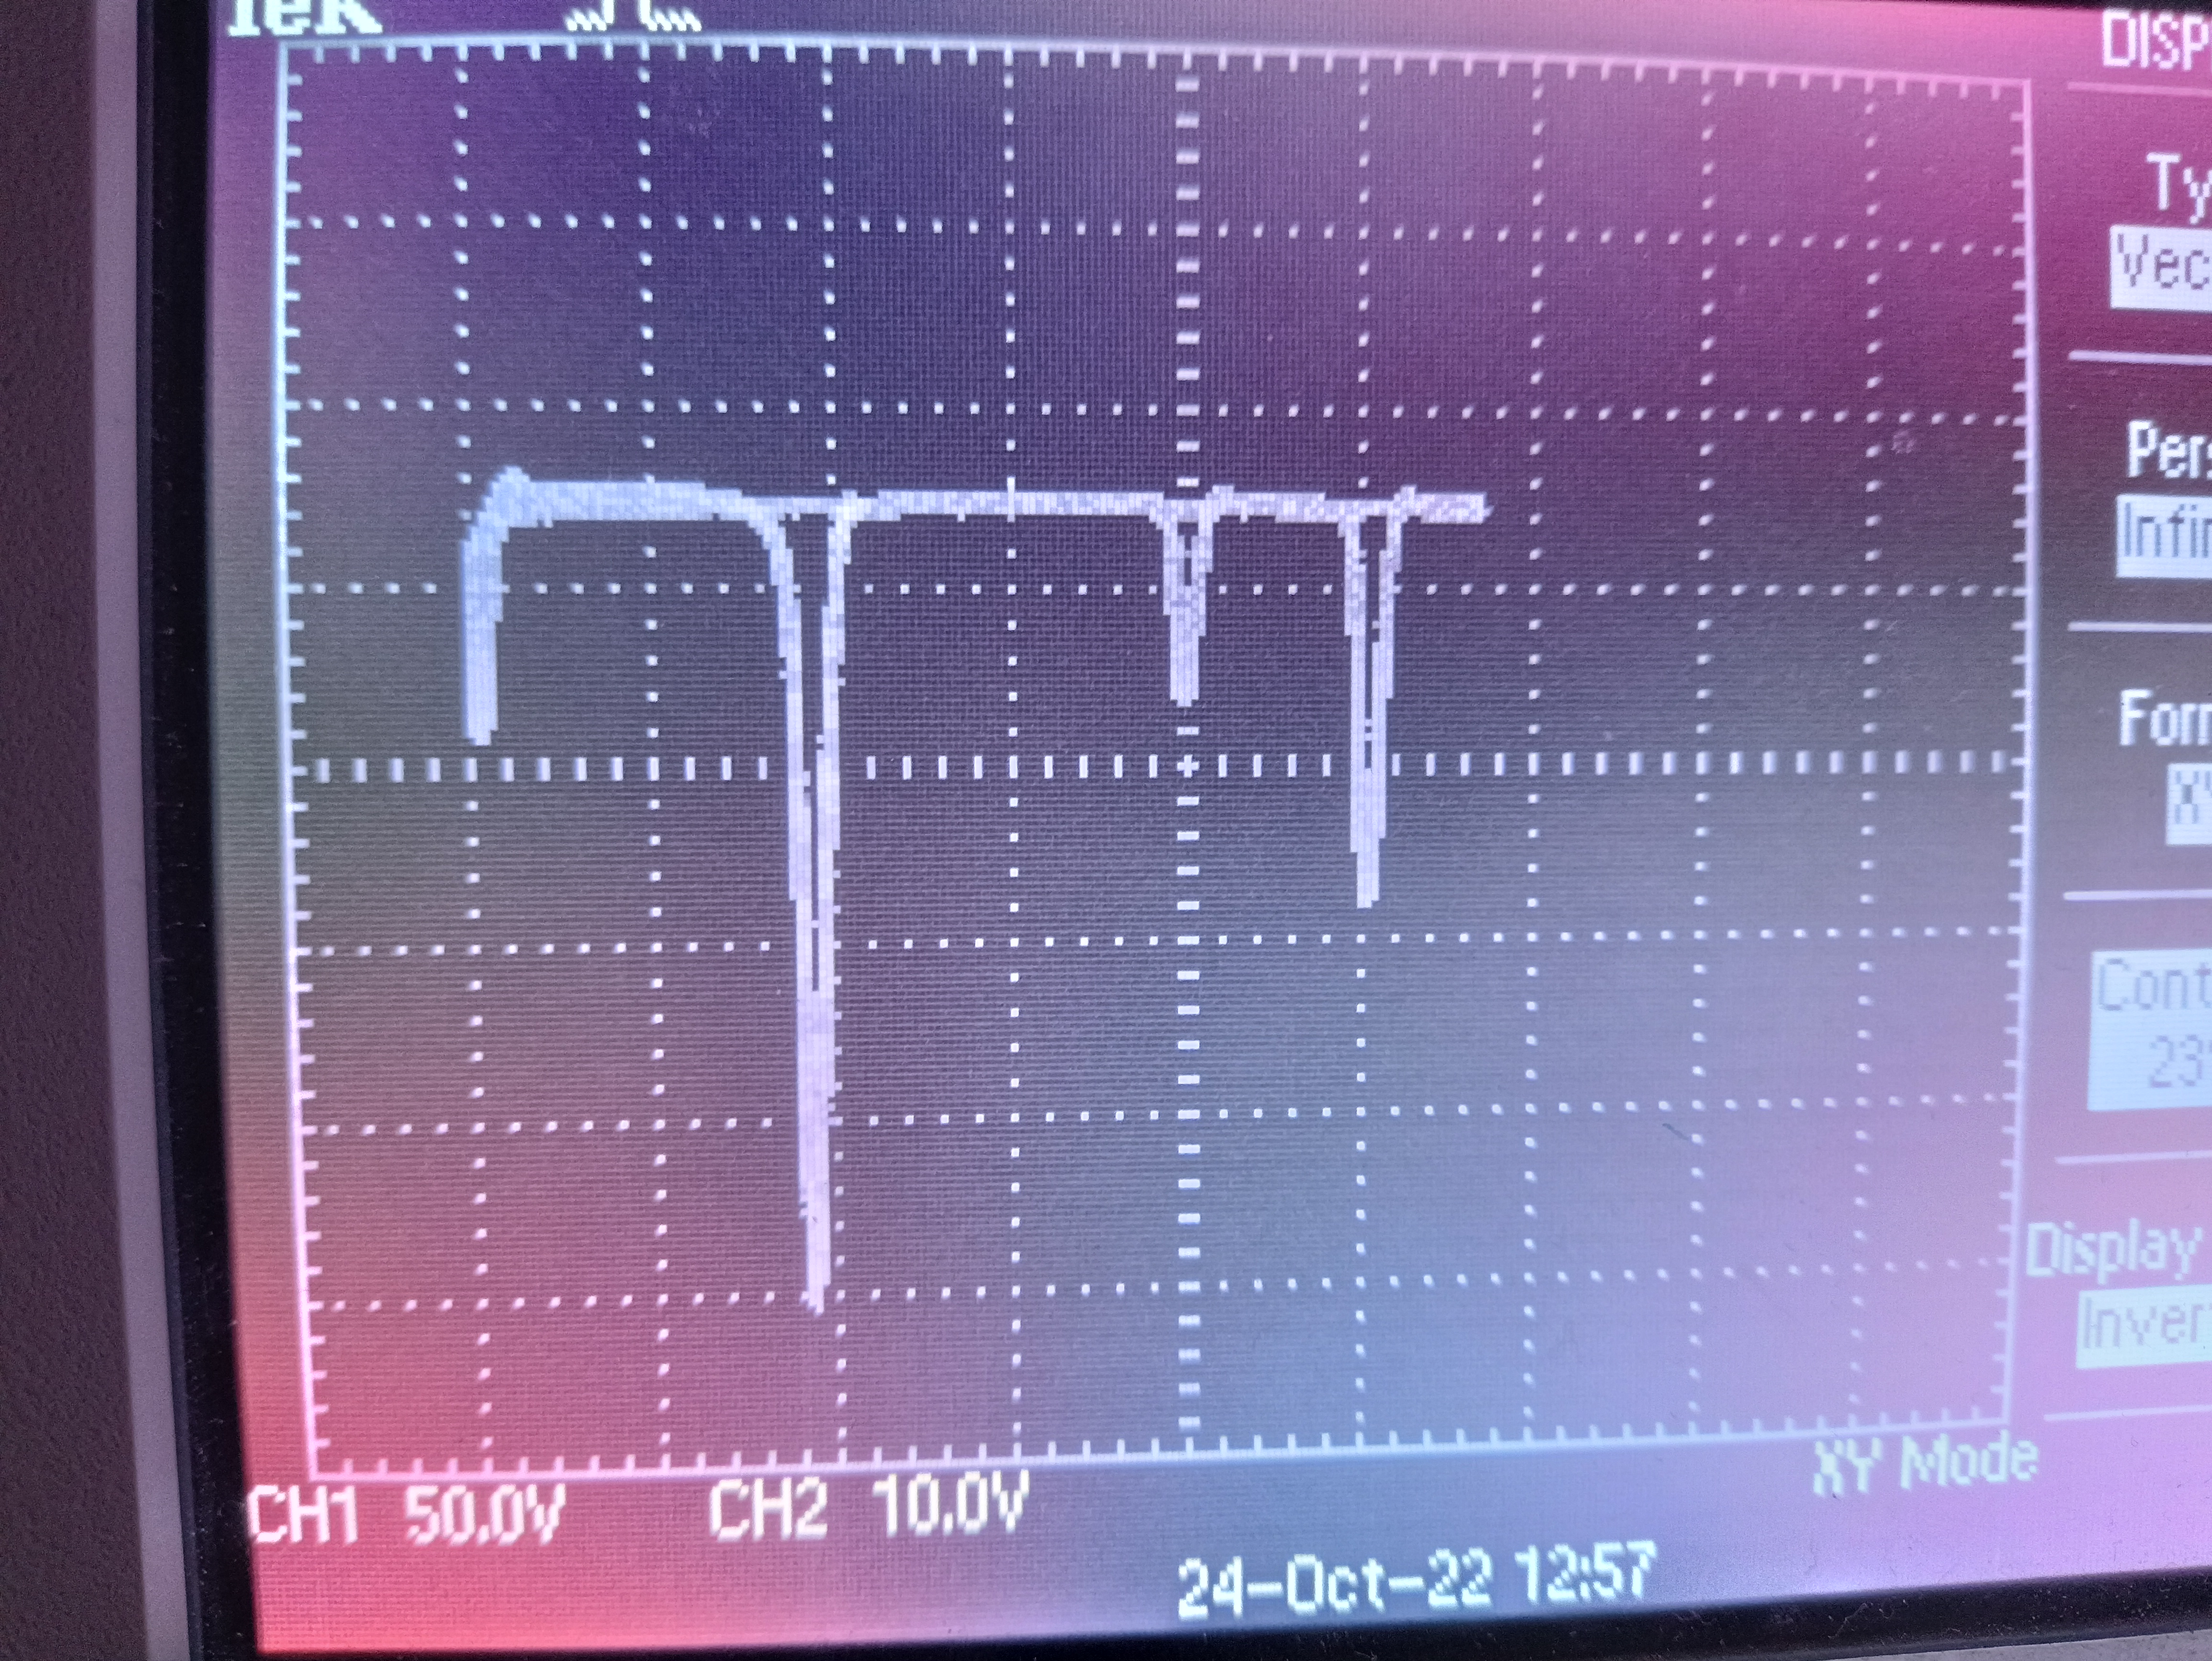
\includegraphics[width=.7\textwidth]{Fotos/Isotopenverhaeltnis.jpg}
    \caption{Foto des Oszilloskops, auf dem ein typisches Signalbild aufgezeichnet ist. Aus dem Verhältnis der beiden rechten Ausschläge lässt sich das Isotopenverhältnis abschätzen.}
    \label{fig:Iso}
\end{figure}

In Abbildung \ref{fig:Iso} ist ein typisches Signalbild abgebildet.
Dabei handelt es sich bei den Ausschlägen um die Resonanzen.
Die beiden rechten Resonanzen sind mit den Isotopen zu identifizieren. 
Die erste von den beiden Resonanzen wird von dem  $^{87}$Rb und die zweite von dem $^{85}$Rb verursacht.
Um das Isotopenverhältnis der in dem Gas befindlichen Rb-Isotope zu bestimmen, kann das Verhältnis der beiden Ausschläge verwendet werden.
Das Verhältnis beläuft sich auf 
\begin{equation*}
    \frac{^{87}\text{Rb}}{^{85}\text{Rb}} = \frac{1}{2}.
\end{equation*}
Damit setzt sich das Gasgemisch zu \nicefrac{1}{3} aus $^{87}$Rb und zu \nicefrac{2}{3} aus $^{85}$Rb zusammen.


\subsection{Quadratischer Zeeman-Effekt}
Über Gleichung REF lässt sich unter Beachtung des quadratischen Terms die Zeeman-Aufspaltung bestimmen. 
Dabei liegt die Hyperfeinaufspaltung des Grundzustandes von $^{87}$Rb bei $\Delta E_{\text{Hyper}}=\SI{4.53e-24}{\joule}$ und von $^{85}$Rb bei $\Delta E_{\text{Hyper}}=\SI{2.01e-24}{\joule}$.
Da der quadratische Term mit der Stärke des Magnetfeldes an Gewicht zunimmt, wird die jeweils größte verwendete magnetische Flussdichte ($^{87}$Rb: \SI{167.21}{\micro\tesla}, $^{85}$Rb: \SI{155.39}{\micro\tesla}) für die Berechnung verwendet.
Damit lässt sich die Energieaufspaltung für $^{87}$Rb ($M_F = 2$) zu 
\begin{equation*}
    \Delta E_{\text{Zeeman}} = \SI{4.8(8)}{\nano\eV}
\end{equation*}
und für $^{85}$Rb ($M_F = 3$) zu 
\begin{equation}
    \Delta E_{\text{Zeeman}} = \SI{4.57(4)}{\nano\eV}
\end{equation}
abschätzen.



\subsection{Periodisches RF-Feld}

\begin{figure}
    \centering
    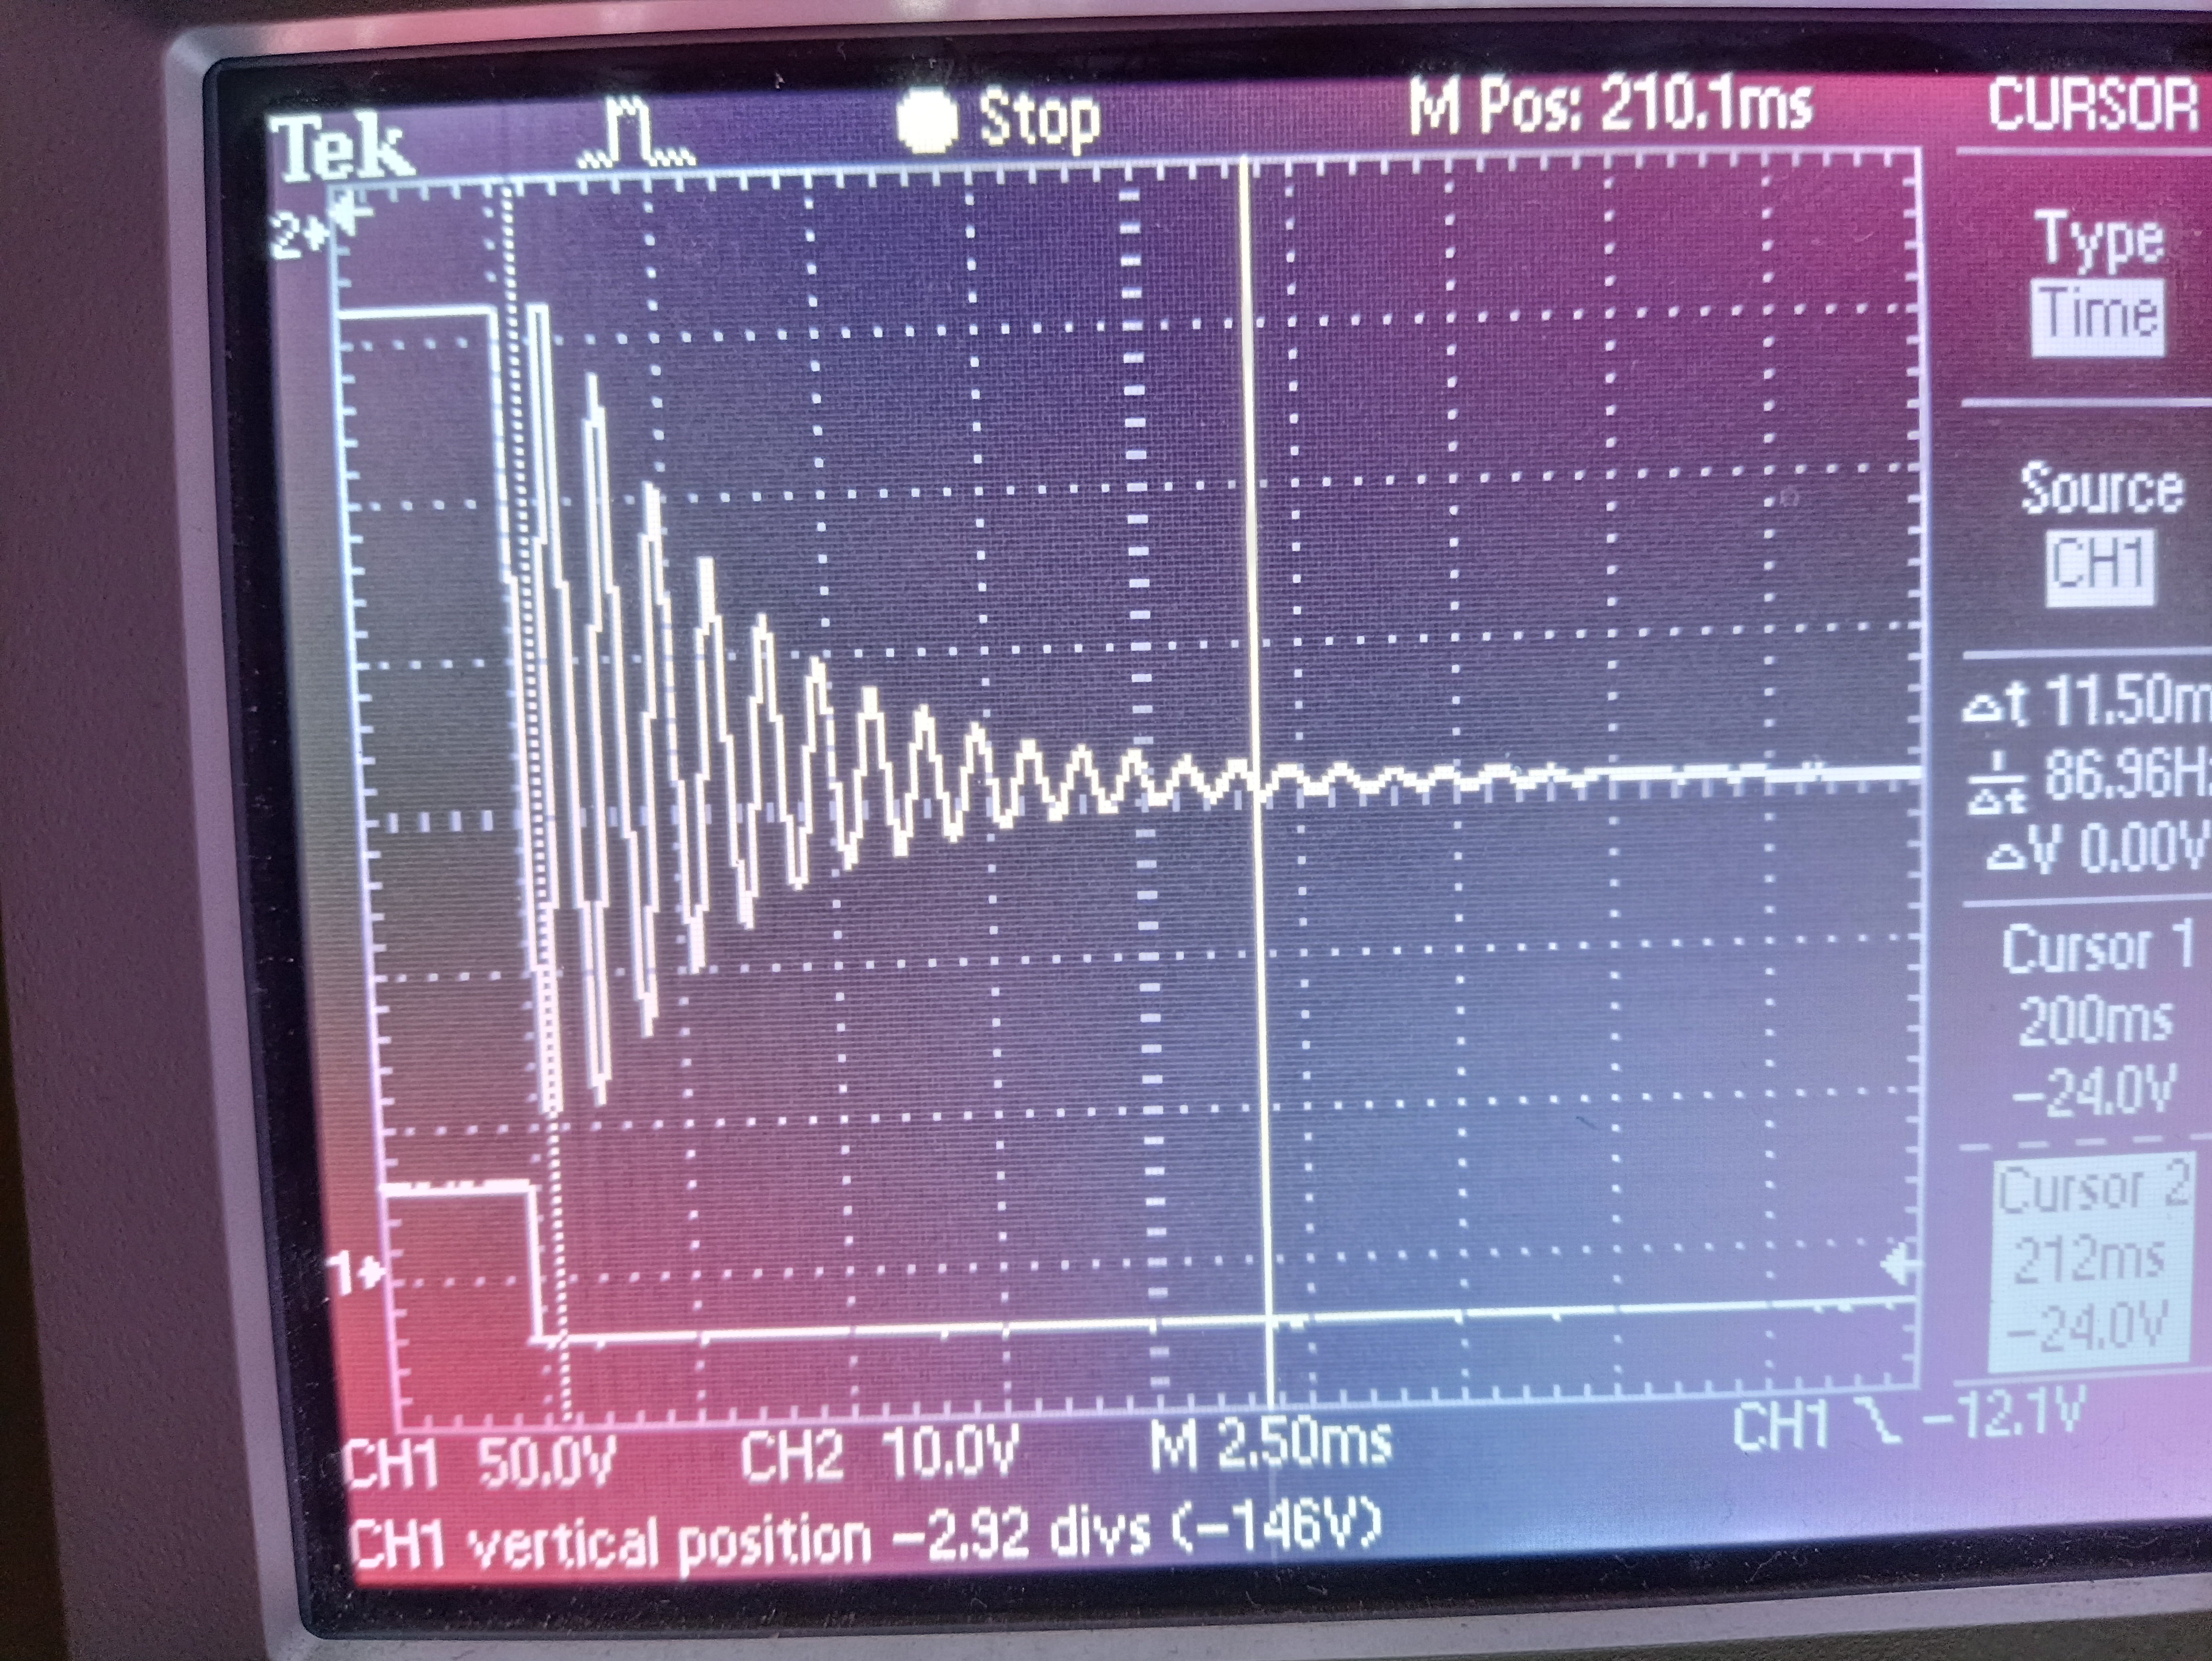
\includegraphics[width=.7\textwidth]{Fotos/Schwingung.jpg}
    \caption{Foto eines Oszilloskops, auf dem ein typischer Signalverlauf im Bereich nach Abschaltung des RF-Feldes abgebildet ist.}
    \label{fig:period_foto}
\end{figure}


Wie in Abschnitt REF beschrieben, wird das RF-Feld periodisch erzeugt.
Zuerst wird der Bereich nach dem Ausschalten des RF-Feldes betrachtet.
Dieser Bereich einer Messung ist in Abbildung \ref{fig:period_foto} dargestellt.
Dort ist eine gedämpfte Oszillation zu erkennen.
Die darüber ermittelten Perioden der Schwingung, in Abhängigkeit der anliegenden RF-Amplitude, sind der Tabelle \ref{tab:period} zu entnehmen.
\begin{table}
    \centering
    \caption{Periodendauern bei unterschiedlichen RF-Feld-Amplituden.}
    \label{tab:period}
    \sisetup{table-format = 1.2}
    \begin{tabular}{S S S}
        \toprule
        {$U \mathbin{/} \si{\volt} $} & {$^{87}$Rb: $T \mathbin{/} \si{\milli\s}$} & {$^{85}$Rb: $T \mathbin{/} \si{\milli\s}$} \\
        \midrule
        1.0     & 4.40    & 6.00    \\
        1.5     & 2.83    & 4.30    \\
        2.0     & 2.17    & 3.20    \\
        2.5     & 1.74    & 2.65    \\
        3.0     & 1.45    & 2.12    \\
        3.5     & 1.26    & 1.86    \\
        4.0     & 1.11    & 1.45    \\
        4.5     & 0.97    & 1.50    \\
        5.0     & 0.88    & 1.31    \\
        6.0     & 0.76    & 1.13    \\
        7.0     & 0.65    & 0.98    \\
        8.0     & 0.56    & 0.85    \\
        9.0     & 0.51    & 0.74    \\
        10.0    & 0.45    & 0.69    \\
        \bottomrule

    \end{tabular}
\end{table}

In Abbildung \ref{fig:period_graf} sind die Periodendauern in Abhängigkeit der RF-Feld-Amplituden grafisch aufgetragen.
Es ist ein hyperbolischer Verlauf zu erkennen. 
Die Messdaten werden mit einer Funktion der Form
\begin{equation}
    T(U) = a+\frac{b}{U-c}
\end{equation}
gefittet.
Die Fitparameter sind in Tabelle \ref{tab:fit_param} aufgeführt.


\begin{figure}
    \centering
    \includegraphics[width=.9\textwidth]{build/Perioden.pdf}
    \caption{Periodendauern in Abhängigkeit der RF-Feld-Amplituden. In die Messwerte lässt sich eine hyperbolische Ausgleichsfunktion legen.}
    \label{fig:period_graf}
\end{figure}

\begin{table}
    \centering
    \caption{Fitparameter der hyperbolischen Ausgleichsfunktion.}
    \label{tab:fit_param}
    \sisetup{table-format = 1.2}
    \begin{tabular}{S| S S S}
        \toprule
        {\text{Isotop}} & {$a \mathbin{/} \si{\milli\s}$} & {$b \mathbin{/} \si{\milli\volt\s}$} & {$c \mathbin{/} \si{\volt}$} \\
        \midrule
        $^{87}$\text{Rb}    &   \num{0.059(16)} & \num{4.07(8)} & \num{0.059(18)} \\
        $^{85}$\text{Rb}    &  \num{-0.02(7)} & \num{6.9(4)} & \num{-0.14(6)} \\
          
        \bottomrule

    \end{tabular}
\end{table}

Die beiden $b$-Parameter können in ein Verhältnis gesetzt werden, welches sich zu
\begin{equation*}
    \frac{b_{85}}{b_{87}} = \num{1.69(10)} 
\end{equation*}
ergibt.





Als Zweites wird der Bereich nach dem Einschalten des RF-Feldes betrachtet. 
In Abbildung \ref{fig:expo_foto} ist wieder ein typischer Signalverlauf abgebildet.
Es handelt sich offensichtlich um einen exponentiellen Anstieg.
In Abbildung \ref{fig:expo_graf} sind die abgelesenen Werte und die jeweiligen exponentiellen Ausgleichsfunktionen der Form
\begin{equation*}
    U = A + b e^{c t}
\end{equation*}
dargestellt.

\begin{figure}
    \centering
    \includegraphics[width=.9\textwidth]{build/Expo.pdf}
    \caption{Spannung in Abhängigkeit der Zeit nach dem Einschalten des RF-Feldes. In die Werte lässt sich eine exponentielle Ausgleichsfunktion legen.}
    \label{fig:expo_graf}
\end{figure}

\begin{figure}
    \centering
    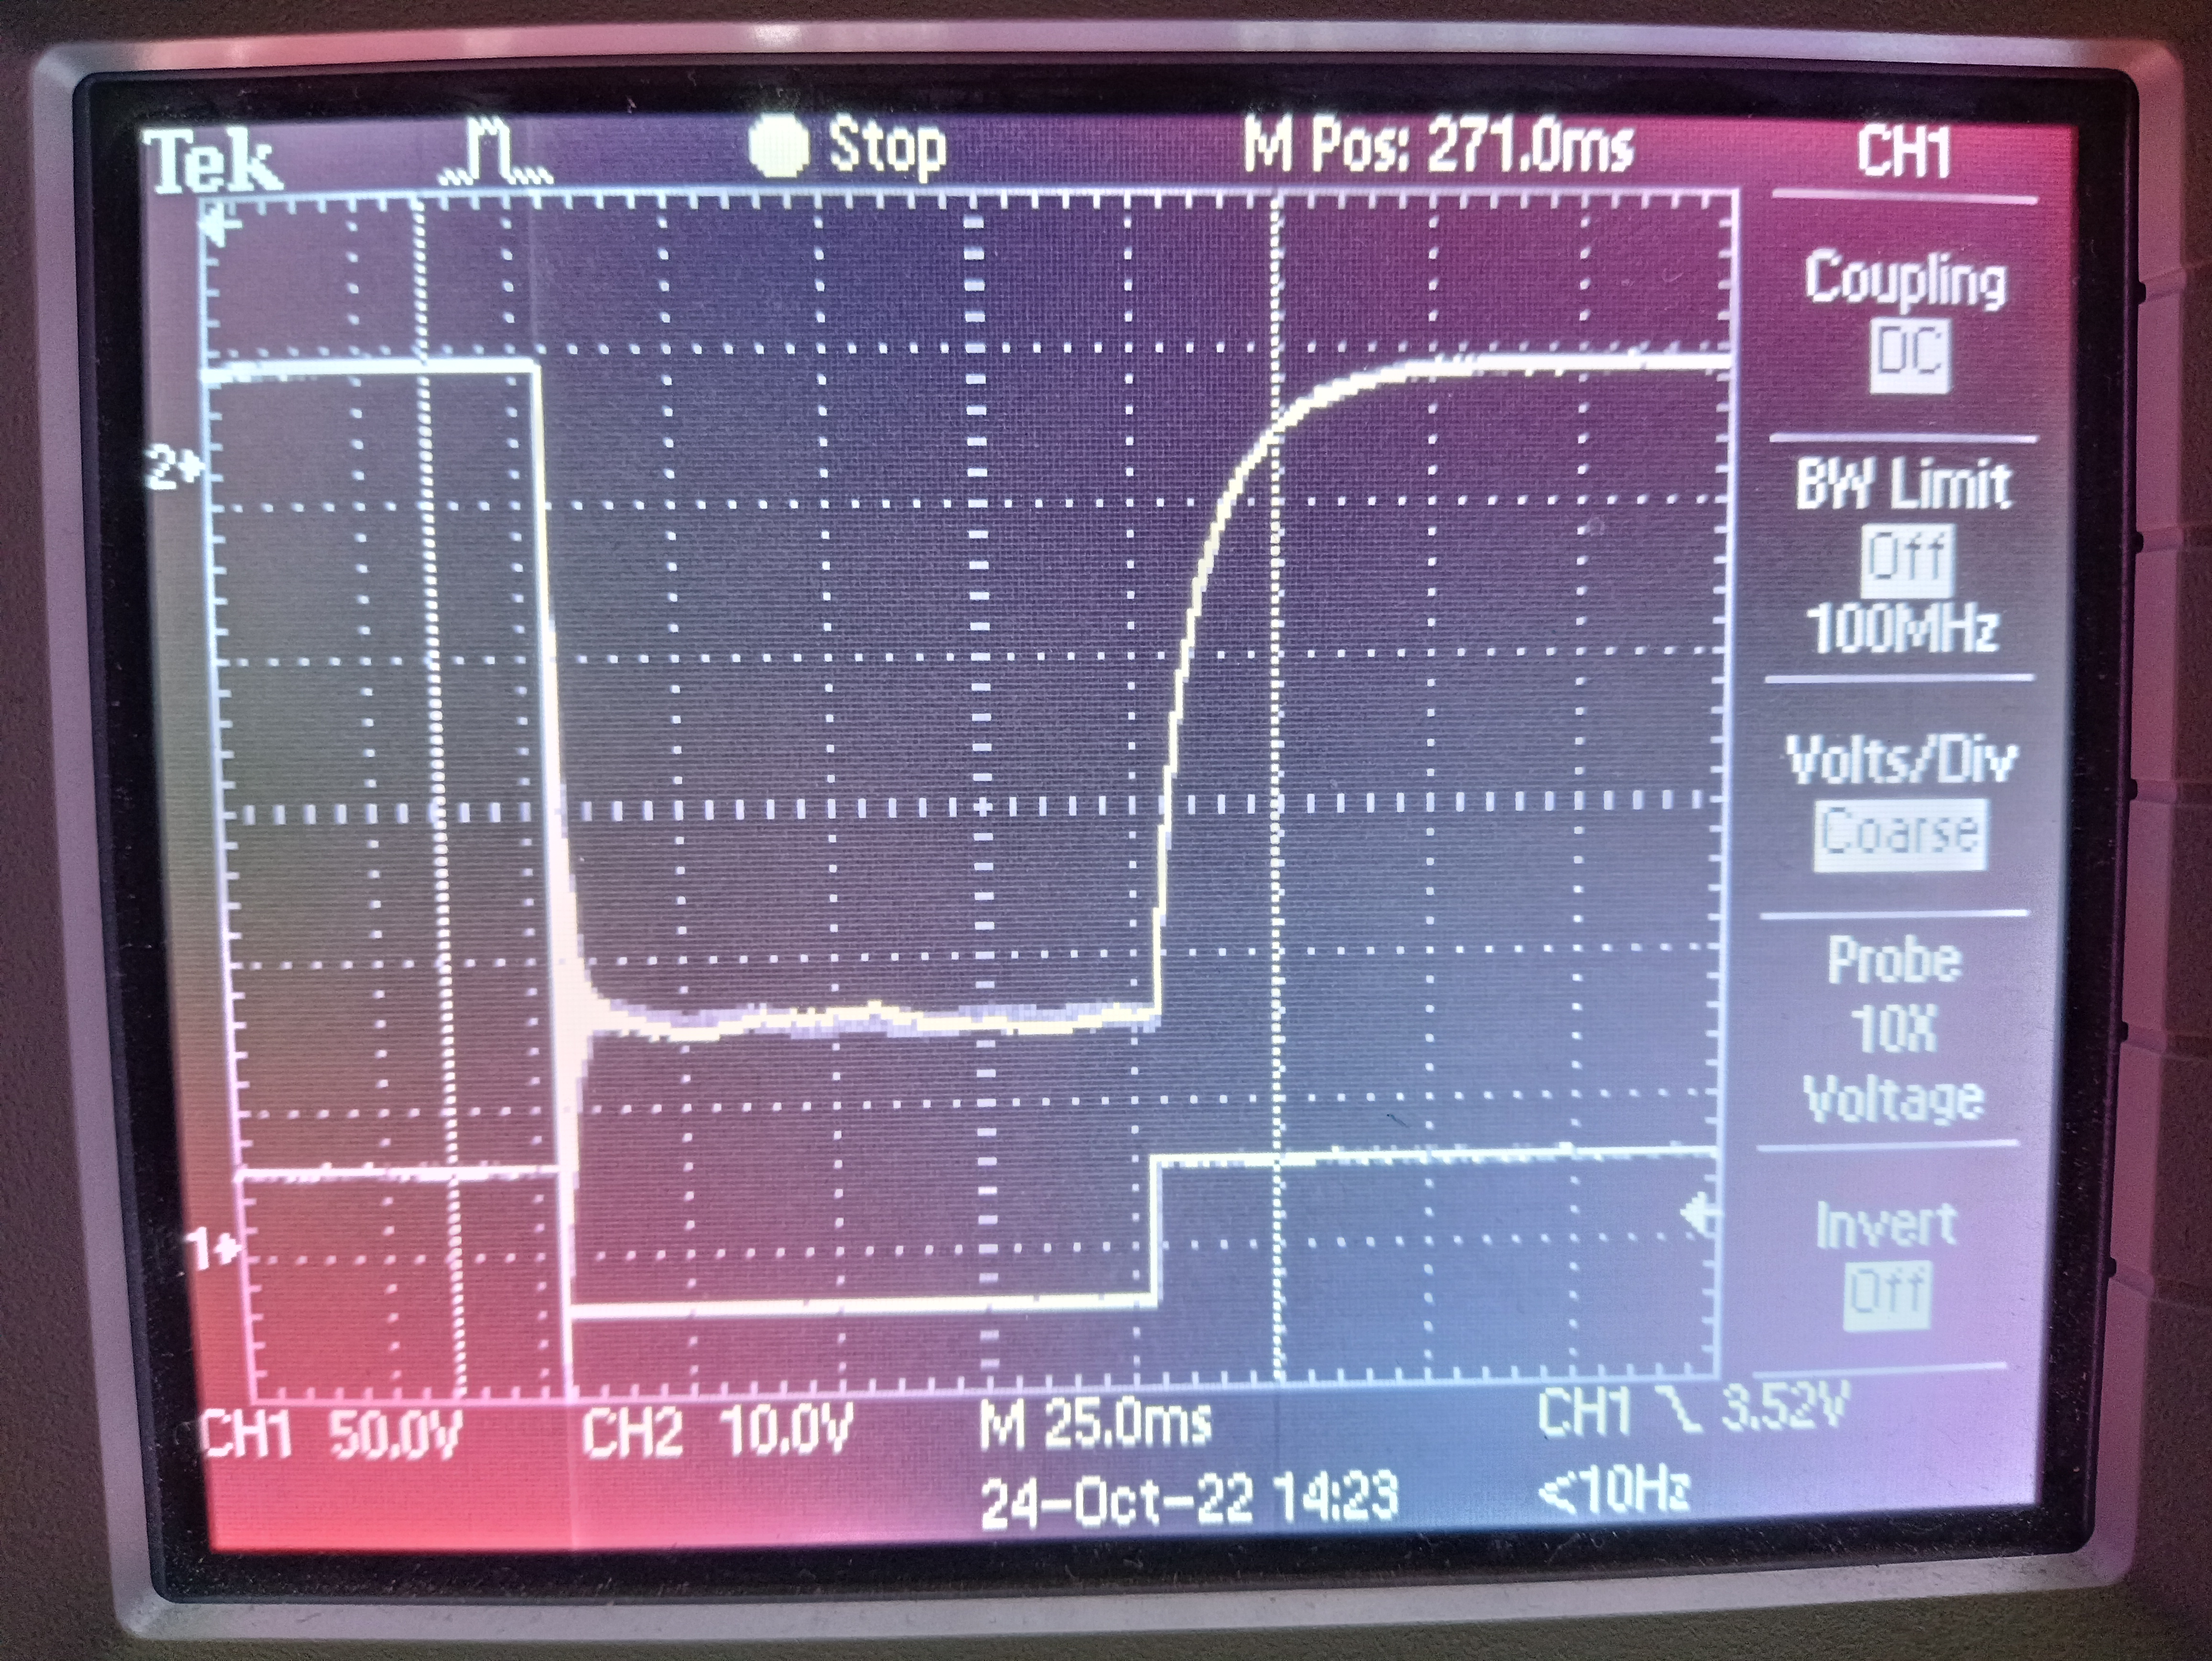
\includegraphics[width=.7\textwidth]{Fotos/Expo_Anstieg.jpg}
    \caption{Foto eines Oszilloskops, auf dem ein typischer Signalverlauf im Bereich nach dem Einschalten des RF-Feldes abgebildet ist.}
    \label{fig:expo_foto}
\end{figure}
% subsection  (end)
%Messwerte: Alle gemessenen physikalischen Größen sind übersichtlich darzustellen.
%
%Auswertung:
%Berechnung der geforderten Endergebnisse
%mit allen Zwischenrechnungen und Fehlerformeln, sodass die Rechnung nachvollziehbar ist.
%Eine kurze Erläuterung der Rechnungen (z.B. verwendete Programme)
%Graphische Darstellung der Ergebnisse